%%%%%%%%%%%%%%%%%%%%%%%%%%%%%%%%%%%%%%%%%%%%%%%%%%%%%%%%%%%%%%%%%%%%%%%%%%%%%%%%
%                         FORMATO DE TESIS FI UNAM                             %
%%%%%%%%%%%%%%%%%%%%%%%%%%%%%%%%%%%%%%%%%%%%%%%%%%%%%%%%%%%%%%%%%%%%%%%%%%%%%%%%
% based on Harish Bhanderi's PhD/MPhil template, then Uni Cambridge
% http://www-h.eng.cam.ac.uk/help/tpl/textprocessing/ThesisStyle/
% corrected and extended in 2007 by Jakob Suckale, then MPI-iCBG PhD programme
% and made available through OpenWetWare.org - the free biology wiki

%                     Under GNU License

% ADAPTADO PARA FI-UNAM:  Jesús Velázquez y Marco Ruiz

\documentclass[twoside,11pt]{Latex/Classes/PhDthesisPSnPDF}
%         PUEDEN INCLUIR EN ESTE ESPACIO LOS PAQUETES EXTRA, O BIEN, EN EL ARCHIVO "PhDthesisPSnPDF.cls" EN "./Latex/Classes/"

\usepackage{blindtext}                     % Para insertar texto Lorem ipsum a traves de la etiqueta \blindtext.
\usepackage[]{algorithm2e}                 % Paquete para ulitizar pseudocódigo.

% This file contains macros that can be called up from connected TeX files
% It helps to summarise repeated code, e.g. figure insertion (see below).

%%%%%%%%%%%%%%%%%%%%%%%%%%%%%%%%%%%%%%%%%%%%%%
%            Colores de la UNAM              %
%%%%%%%%%%%%%%%%%%%%%%%%%%%%%%%%%%%%%%%%%%%%%%
%Azul Pantone 541  -->(0,63,119) RGB
\definecolor{Azul}{RGB}{0,63,119}

%Oro Pantone 460  -->(234,221,150) RGB
\definecolor{Oro}{RGB}{234,221,150}


%%%%%%%%%%%%%%%%%%%%%%%%%%%%%%%%%%%%%%%%%%%%%%
%            Comandos para líneas            %
%%%%%%%%%%%%%%%%%%%%%%%%%%%%%%%%%%%%%%%%%%%%%%
%Se define un comando \colorvrule para hacer líneas verticales de color con 3 argumentos: color, ancho, alto
\newcommand{\colorvrule}[3]{
\begingroup\color{#1}\vrule width#2 height#3
\endgroup}

%Se define un comando \colorhrule para hacer líneas horizontales de color con 2 argumentos: color, ancho
\newcommand{\colorhrule}[2]{
\begingroup\color{#1}\hrule height#2
\endgroup}

%%%%%%%%%%%%%%%%%%%%%%%%%%%%%%%%%%%%%%%%%%%%%%
%          Comando para derivadas            %
%%%%%%%%%%%%%%%%%%%%%%%%%%%%%%%%%%%%%%%%%%%%%%
\newcommand{\derivada}[3][]{\ensuremath{\dfrac{\mbox{d}^{#1}#2}{\mbox{d}#3^{#1}}}} 
%primer argumento(opcional): orden de la derivada
%segundo argumento: función a derivar
%tercer argumento: variable respecto a la que se deriva


%%%%%%%%%%%%%%%%%%%%%%%%%%%%%%%%%%%%%%%%%%%%%%
%       Comando para la exponencial          %
%%%%%%%%%%%%%%%%%%%%%%%%%%%%%%%%%%%%%%%%%%%%%%
\newcommand{\e}[1][]{\ensuremath{\mbox{e}^{#1}}}
%primer argumento(opcional): exponente de la exponencial




% insert a centered figure with caption and description
% parameters 1:filename, 2:title, 3:description and label
\newcommand{\figuremacro}[3]{
	\begin{figure}[htbp]
		\centering
		\includegraphics[width=1\textwidth]{#1}
		\caption[#2]{\textbf{#2} - #3}
		\label{condicion}
	\end{figure}
}

% insert a centered figure with caption and description AND WIDTH
% parameters 1:filename, 2:title, 3:description and label, 4: textwidth
% textwidth 1 means as text, 0.5 means half the width of the text
\newcommand{\figuremacroW}[4]{
	\begin{figure}[htbp]
		\centering
		\includegraphics[width=#4\textwidth]{#1}
		\caption[#2]{\textbf{#2} - #3}
		\label{#1}
	\end{figure}
}

% inserts a figure with wrapped around text; only suitable for NARROW figs
% o is for outside on a double paged document; others: l, r, i(inside)
% text and figure will each be half of the document width
% note: long captions often crash with adjacent content; take care
% in general: above 2 macro produce more reliable layout
\newcommand{\figuremacroN}[3]{
	\begin{wrapfigure}{o}{0.5\textwidth}
		\centering
		\includegraphics[width=0.48\textwidth]{#1}
		\caption[#2]{{\small\textbf{#2} - #3}}
		\label{#1}
	\end{wrapfigure}
}

% predefined commands by Harish
\newcommand{\PdfPsText}[2]{
  \ifpdf
     #1
  \else
     #2
  \fi
}

\newcommand{\IncludeGraphicsH}[3]{
  \PdfPsText{\includegraphics[height=#2]{#1}}{\includegraphics[bb = #3, height=#2]{#1}}
}

\newcommand{\IncludeGraphicsW}[3]{
  \PdfPsText{\includegraphics[width=#2]{#1}}{\includegraphics[bb = #3, width=#2]{#1}}
}

\newcommand{\InsertFig}[3]{
  \begin{figure}[!htbp]
    \begin{center}
      \leavevmode
      #1
      \caption{#2}
      \label{#3}
    \end{center}
  \end{figure}
}







%%% Local Variables:
%%% mode: latex
%%% TeX-master: "~/Documents/LaTeX/CUEDThesisPSnPDF/thesis"
%%% End:
          % Archivo con funciones útiles

%%%%%%%%%%%%%%%%%%%%%%%%%%%%%%%%%%%%%%%%%%%%%%%%%%%%%%%%%%%%%%%%%%%%%%%%%%%%%%%%
%                                   DATOS                                      %
%%%%%%%%%%%%%%%%%%%%%%%%%%%%%%%%%%%%%%%%%%%%%%%%%%%%%%%%%%%%%%%%%%%%%%%%%%%%%%%%
\title{Título de la tesis}
\author{Julio César Guzmán Villanueva}        
\degree{Ingeniero en Computación}           % Carrera
\director{Ing. Stalin Muñoz Gutierrez}      % Director de tesis
\degreedate{2015}                           % Año de la fecha del examen
\lugar{México, D.F.}                        % Lugar
%\portadafalse                              % Portada en NEGRO, descomentar y comentar la línea siguiente si se quiere utilizar
\portadatrue                                % Portada en COLOR

\keywords{tesis,autor,tutor,etc}            % Palablas clave para los metadatos del PDF
\subject{tema_1,tema_2}                     % Tema para metadatos del PDF  

%%%%%%%%%%%%%%%%%%%%%%%%%%%%%%%%%%%%%%%%%%%%%%%%%%%%%
%                   PORTADA                         %
%%%%%%%%%%%%%%%%%%%%%%%%%%%%%%%%%%%%%%%%%%%%%%%%%%%%%
\begin{document}

\begin{titlepage}
\maketitle
\end{titlepage}

%%%%%%%%%%%%%%%%%%%%%%%%%%%%%%%%%%%%%%%%%%%%%%%%%%%%%
%                  PRÓLOGO                          %
%%%%%%%%%%%%%%%%%%%%%%%%%%%%%%%%%%%%%%%%%%%%%%%%%%%%%
\frontmatter
\begin{dedication}
A la Facultad de Ingeniería y a la  Universidad, por la formación que me han dado.\\
Es gracias a ustedes que es posible el presente trabajo.\\
En verdad, gracias.\\
Yo.
\end{dedication}
       % Comentar línea si no se usa
%\chapter*{}
%\pagenumbering{Roman}

\begin{acknowledgements}



\end{acknowledgements}




   % Comentar línea si no se usa 
% ******************************* Thesis Declaration ********************************

\begin{declaration}

Por la presente declaro que, salvo cuando se haga referencia específica al trabajo de otras personas, el contenido de esta tesis es original y no se ha presentado total o parcialmente para su consideración para cualquier otro título o grado en esta o cualquier otra Universidad. Esta tesis es resultado de mi propio trabajo y no incluye nada que sea el resultado de algún trabajo realizado en colaboración, salvo que se indique específicamente en el texto. 
% Author and date will be inserted automatically from thesis.tex
\end{declaration}
           % Comentar línea si no se usa

% Thesis Abstract -----------------------------------------------------


%\begin{abstractslong}    %uncommenting this line, gives a different abstract heading
\begin{abstracts}        %this creates the heading for the abstract page

\blindtext

\end{abstracts}
%\end{abstractlongs}


% ----------------------------------------------------------------------                   % Comentar línea si no se usa

%%%%%%%%%%%%%%%%%%%%%%%%%%%%%%%%%%%%%%%%%%%%%%%%%%%%%
%                   ÍNDICES                         %
%%%%%%%%%%%%%%%%%%%%%%%%%%%%%%%%%%%%%%%%%%%%%%%%%%%%%
%Esta sección genera el índice
\setcounter{secnumdepth}{3} % organisational level that receives a numbers
\setcounter{tocdepth}{3}    % print table of contents for level 3
\tableofcontents            % Genera el índice 
%: ----------------------- list of figures/tables ------------------------
\listoffigures              % Genera el ínidce de figuras, comentar línea si no se usa
\listoftables               % Genera índice de tablas, comentar línea si no se usa

%%%%%%%%%%%%%%%%%%%%%%%%%%%%%%%%%%%%%%%%%%%%%%%%%%%%%
%                   CONTENIDO                       %
%%%%%%%%%%%%%%%%%%%%%%%%%%%%%%%%%%%%%%%%%%%%%%%%%%%%%
% the main text starts here with the introduction, 1st chapter,...
\mainmatter
\def\baselinestretch{1.5}                   % Interlineado de 1.5

% this file is called up by thesis.tex
% content in this file will be fed into the main document
%----------------------- introduction file header -----------------------
%%%%%%%%%%%%%%%%%%%%%%%%%%%%%%%%%%%%%%%%%%%%%%%%%%%%%%%%%%%%%%%%%%%%%%%%%
%  Capítulo 1: Introducción- DEFINIR OBJETIVOS DE LA TESIS              %
%%%%%%%%%%%%%%%%%%%%%%%%%%%%%%%%%%%%%%%%%%%%%%%%%%%%%%%%%%%%%%%%%%%%%%%%%

\chapter{Introducción}

%: ----------------------- HELP: latex document organisation
% the commands below help you to subdivide and organise your thesis
%    \chapter{}       = level 1, top level
%    \section{}       = level 2
%    \subsection{}    = level 3
%    \subsubsection{} = level 4
%%%%%%%%%%%%%%%%%%%%%%%%%%%%%%%%%%%%%%%%%%%%%%%%%%%%%%%%%%%%%%%%%%%%%%%%%
%                           Presentación                                %
%%%%%%%%%%%%%%%%%%%%%%%%%%%%%%%%%%%%%%%%%%%%%%%%%%%%%%%%%%%%%%%%%%%%%%%%%

\section{Presentación}
\blindtext

%%%%%%%%%%%%%%%%%%%%%%%%%%%%%%%%%%%%%%%%%%%%%%%%%%%%%%%%%%%%%%%%%%%%%%%%%
%                           Objetivo                                    %
%%%%%%%%%%%%%%%%%%%%%%%%%%%%%%%%%%%%%%%%%%%%%%%%%%%%%%%%%%%%%%%%%%%%%%%%%

\section{Objetivo}
\blindtext

%%%%%%%%%%%%%%%%%%%%%%%%%%%%%%%%%%%%%%%%%%%%%%%%%%%%%%%%%%%%%%%%%%%%%%%%%
%                  Motivación y estado del arte                         %
%%%%%%%%%%%%%%%%%%%%%%%%%%%%%%%%%%%%%%%%%%%%%%%%%%%%%%%%%%%%%%%%%%%%%%%%%
\section{Motivación}
\blindtext

%%%%%%%%%%%%%%%%%%%%%%%%%%%%%%%%%%%%%%%%%%%%%%%%%%%%%%%%%%%%%%%%%%%%%%%%%
%                   Planteamiento del problema                          %
%%%%%%%%%%%%%%%%%%%%%%%%%%%%%%%%%%%%%%%%%%%%%%%%%%%%%%%%%%%%%%%%%%%%%%%%%
\section{Planteamiento del problema}
\blindtext

%%%%%%%%%%%%%%%%%%%%%%%%%%%%%%%%%%%%%%%%%%%%%%%%%%%%%%%%%%%%%%%%%%%%%%%%%
%                           Metodologia                                 %
%%%%%%%%%%%%%%%%%%%%%%%%%%%%%%%%%%%%%%%%%%%%%%%%%%%%%%%%%%%%%%%%%%%%%%%%%
\section{Metodología} 
\blindtext

%%%%%%%%%%%%%%%%%%%%%%%%%%%%%%%%%%%%%%%%%%%%%%%%%%%%%%%%%%%%%%%%%%%%%%%%%
%                         Contribuciones                                %
%%%%%%%%%%%%%%%%%%%%%%%%%%%%%%%%%%%%%%%%%%%%%%%%%%%%%%%%%%%%%%%%%%%%%%%%%

\section{Contribuciones} %Escribir al final
\blindtext

%%%%%%%%%%%%%%%%%%%%%%%%%%%%%%%%%%%%%%%%%%%%%%%%%%%%%%%%%%%%%%%%%%%%%%%%%
%                           Estructura de la tesis                      %
%%%%%%%%%%%%%%%%%%%%%%%%%%%%%%%%%%%%%%%%%%%%%%%%%%%%%%%%%%%%%%%%%%%%%%%%%

\section{Estructura de la tesis} %Escribir al final
\blindtext

            % ~10 páginas - Explicar el propósito de la tesis
\include{Capitulo2/Marco_teorico}           % ~20 páginas - Poner un contexto a la tesis, hacer referencia a trabajos actuales en el tema

%%%%%%%%%%%%%%%%%%%%%%%%%%%%%%%%%%%%%%%%%%%%%%%%%%%%%%%%%%%%%%%%%%%%%%%%%
%           Capítulo 3: NOMBRE                   %
%%%%%%%%%%%%%%%%%%%%%%%%%%%%%%%%%%%%%%%%%%%%%%%%%%%%%%%%%%%%%%%%%%%%%%%%%

\chapter{Diseño del experimento}
En este capítulo, se presenta la introducción al desarrollo de la tesis, ya sea el modelo matemático o las bases del proyecto, etc.

\section{Sección}
    \subsection{Subsección}
        \blindtext
        
\subsection{Subsección}
    \Blindtext
  % ~20 páginas - Explicar el problema en específico que se va a resolver, la metodología y experimentos métodos utilizados
\chapter{Análisis de Resultados}

    \section{Resultados}
    


    \section{Comparación con otros algoritmos}
    
   % ~20 páginas - Presentar los resultados tal cual son, y analizarlos.
\include{Capitulo5/Conclusiones}            % ~5 páginas - Resumir lo que se hizo y lo que no y comentar trabajos futuros sobre el tema

%%%%%%%%%%%%%%%%%%%%%%%%%%%%%%%%%%%%%%%%%%%%%%%%%%%%%
%                   APÉNDICES                       %
%%%%%%%%%%%%%%%%%%%%%%%%%%%%%%%%%%%%%%%%%%%%%%%%%%%%%
\appendix
% this file is called up by thesis.tex
% content in this file will be fed into the main document
\chapter{Apendice ejemplos de \LaTeX}
% top level followed by section, subsection

    \section{\textcolor{Azul}{Ejemplo de sección en color azul}}

    \section{Ejemplo de tablas}

        Antes de comenzar, se definen  en la tabla ~\ref{tab:tabla} los parámetros y variables utilizadas

        %%%%%%%%Tabla Nombres de parámetros
        \begin{table}[htdp]                             %Inicia el entorno table debajo del texto
            \centering\                                     %   centra la tabla
                \begin{tabular}{||c | c ||}                     %inicia entorno tabular con doble línea en las orillas, 2 columnas con el contenido centrado (c)
                \hline                                          %inserta línea horizontal
                \hline
                Nombre Parámetro/Variable & Símbolo\\
                \hline
                \hline
                Masa del péndulo & $m$ \\
                \hline
                Masa del carro & $M$\\
                \hline
                Distancia del eje de giro al centro de masa & $l$ \\
                \hline
                Aceleración gravitatoria & $g$ \\
                \hline
                Momento de inercia péndulo respecto del eje de giro& $J$ \\
                \hline
                Ángulo del péndulo respecto del eje vertical & $\theta$\\
                \hline
                Velocidad angular del péndulo & $\dot{\theta}$, $\omega$\\
                \hline
                Distancia del carro respecto al centro del riel & x\\
                \hline
                Velocidad del carro & $\dot{x}$, $v$\\
                \hline
                \hline
                \end{tabular}
            \caption[Parámetros dinámicos del carro-péndulo]{\textbf{Parámetros dinámicos del carro-péndulo} - Estos son los valores de parámetros utilizados en el diseño y las simulaciones, corresponden a los valores reales.}
            \label{tab:tabla}                              %etiqueta para referencia
        \end{table}

    \section{Ejemplo de MATLAB (según Jesús)}

        %inserción de codigo de Matlab
        %Es conveniente sangrarlo (los de proteco dicen "indentarlo") para que no se encime con los números  de las líneas a la izquierda

        \begin{lstlisting}[frame=single]
        
            % Declaracion de las variables simbolicas
            syms u z1 z2 z3 z4 J m M g l 
            % Matrices involucradas
            E = [J+m*l*l m*l*cos(z1);m*l*cos(z1) M+m] 
            F = [m*g*l*sin(z1);u+m*l*(z3*z3)*sin(z1)] 
            % Despeje
            V = E\F
            
        \end{lstlisting}


    \section{Ejemplo de citas}

        Ejemplo de cita 1 \cite{latex}


        Ejemplo de cita 2 \cite{prime-number-theorem}
        
        
        Ejemplo de cita 3 \cite{WinNT}

    \section{Ejemplo de pseudocódigo}

        \begin{algorithm}[H]
            \KwData{this text}
            \KwResult{how to write algorithm with \LaTeX2e }
            initialization\;
            \While{not at end of this document}
            {
                read current\;
                \eIf{understand}
                {
                   go to next section\;
                   current section becomes this one\;
                }
                {
                   go back to the beginning of current section\;
                }
            }
            \caption{How to write algorithms}
        \end{algorithm}

    \section{Ejemplo de figuras}

        La figura ~\ref{fig:planta}    % Hace referencia a la imagen "planta" el número se inserta automáticamente
        ilustra los compenentes de la planta.

        \begin{figure}
          \centering
            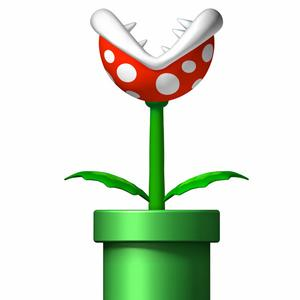
\includegraphics[scale=0.5]{Apendice1/figs/planta.jpg}      % Ruta completa de la imagen, porque se compila desde el archivo tesis.tex
            \caption{Descripción de la planta}            %Pie de imagen
            \label{fig:planta}                            %nombre de referencia
        \end{figure}
        
        \section{Matrices and other arrays in \LaTeX}
            Matrices and other arrays are produced in LaTeX using the \textbf{array} environment. For example, suppose that we wish to typeset the following passage:\\
            The \emph{characteristic polynomial} $\chi(\lambda)$ of the $3 \times 3
            $~matrix
            \[ \left( 
                \begin{array}{ccc}
                    a & b & c \\
                    d & e & f \\
                    g & h & i \end{array} \right)\]


        is given by the formula


            \[ \chi(\lambda) = \left| \begin{array}{ccc}
            \lambda - a & -b & -c \\
            -d & \lambda - e & -f \\
            -g & -h & \lambda - i \end{array} \right|.\] 
            
            
        We can therefore obtain the above formula by typing
        \[ |x| = \left\{ \begin{array}{ll}
                 x & \mbox{if $x \geq 0$};\\
                -x & \mbox{if $x < 0$}.\end{array} \right. \]

% Ejemplo de teoremas

\newtheorem{theorem}{Theorem}[section]
\newtheorem{corollary}{Corollary}[theorem]
\newtheorem{lemma}[theorem]{Lemma}
 

\section{Introduction}
Theorems can easily be defined
 
\begin{theorem}
Let $f$ be a function whose derivative exists in every point, then $f$ is 
a continuous function.
\end{theorem}
 
\begin{theorem}[Pythagorean theorem]
\label{pythagorean}
This is a theorema about right triangles and can be summarised in the next 
equation 
\[ x^2 + y^2 = z^2 \]
\end{theorem}
 
And a consequence of theorem \ref{pythagorean} is the statement in the next 
corollary.
 
\begin{corollary}
There's no right rectangle whose sides measure 3cm, 4cm, and 6cm.
\end{corollary}
 
You can reference theorems such as \ref{pythagorean} when a label is assigned.
 
\begin{lemma}
Given two line segments whose lengths are $a$ and $b$ respectively there is a 
real number $r$ such that $b=ra$.
\end{lemma}

%Agregar en otros archivos.

\chapter{Apendice Matemático}
    \section{Matrices}
    \section{Algebra Lineal}
    \section{Procesos estocasticos}
    \section{Cálculo Vectorial}
    
\chapter{Apendice de Inteligencia Artificial}
    \section{Redes Neuronales}
        \subsection{Perceptron}
        \subsection{Redes neuronales multicapa}
    \section{Agentes}
    \section{Algoritmos geneticos/evolutivos}
        \subsection{NSGA-II}
    \section{Cadenas de Markov}
    \section{Inteligencia de colmena}
    \section{Análisis de sentimiento}
    \section{Rationality}
    
\chapter{Apendice de Game Theory}
    \section{Game Theory} 
    \section{Types of games}
        \subsection{Cooperative or non-cooperative}
        \subsection{Symmetric and asymmetric}
        \subsection{Zero-sum and non-zero-sum}
        \subsection{Simultaneous and sequential}   
        \subsection{Perfect information and imperfect information}
        \subsection{Combinatorial games}
        \subsection{Infinite long games}
        \subsection{Discrete and continuous games}
        \subsection{Differential games}
        \subsection{Many-player and population games}
        \subsection{Stochastic outcomes (and relation to other fields)}
        \subsection{Metagames}
    \section{Collective intentionality}
        
\chapter{Apendice de métodos bayesianos en finanzas}
    \section{Conceptos.(Incluir indice)}               % Colocar los circuitos, manuales, código fuente, pruebas de teoremas, etc.

%%%%%%%%%%%%%%%%%%%%%%%%%%%%%%%%%%%%%%%%%%%%%%%%%%%%%
%                                     %
%%%%%%%%%%%%%%%%%%%%%%%%%%%%%%%%%%%%%%%%%%%%%%%%%%%%%
\begin{small} % tiny(5) < scriptsize(7) < footnotesize(8) < small (9)
\bibliographystyle{Latex/Classes/PhDbiblio-url2}    % Title is link if provided
\bibliography{Bibliografia/Referencias}             % Archivo .bib
\end{small}
% --------------------------------------------------------------
% existen varios estilos de bilbiografía, pueden cambiarlos a placer

% in-text refs: (1) (1; 2)
% ref list: alphabetical; author(s) in small caps; initials last name; page(s)
%\bibliographystyle{Latex/Classes/PhDbiblio-case} % title forced lower case
%\bibliographystyle{Latex/Classes/PhDbiblio-bold} % title as in bibtex but bold
%\bibliographystyle{Latex/Classes/PhDbiblio-url} % bold + www link if provided

%\bibliographystyle{Latex/Classes/jmb} % calls style file jmb.bst
% in-text refs: author (year) without brackets
% ref list: alphabetical; author(s) in normal font; last name, initials; page(s)

%\bibliographystyle{plainnat} % calls style file plainnat.bst
% in-text refs: author (year) without brackets
% (this works with package natbib)
% --------------------------------------------------------------
% according to Dresden med fac summary has to be at the end
%\include{0_frontmatter/abstract}
%: Declaration of originality
%\include{9_backmatter/declaration}

\end{document}